\begin{figure}[t]
\centering
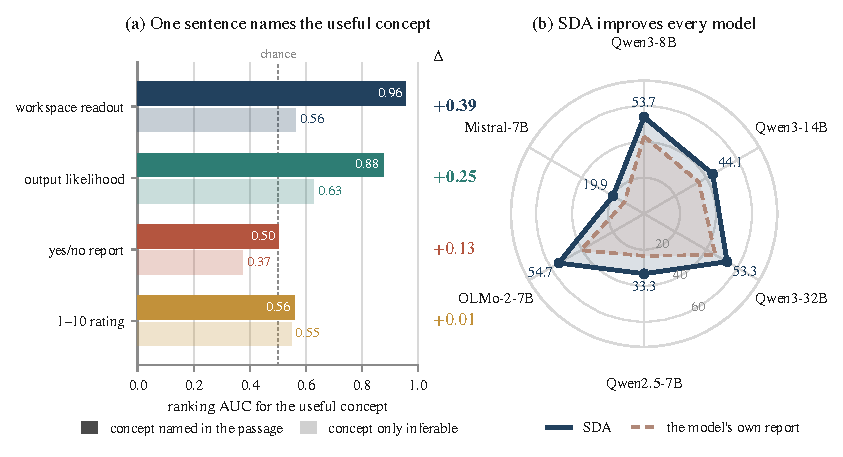
\includegraphics[width=\textwidth]{figures/fig_teaser.pdf}
\caption{\textbf{Naming a concept moves model computation far more than importance reports express;
Self-Distilled Admission (SDA) turns that computation into admission decisions.} (a) Matched episodes,
candidates, labels and questions differ by one sentence naming the otherwise inferable concept.
On the standard Fresh-2 pool, horizontal bars show six-model mean pooled ranking AUC (0--1; dashed chance line, 0.5): named concepts are
solid, inferable concepts pale. Workspace readout rises from 0.563 to 0.956 ($+0.39$), output likelihood
from 0.628 to 0.876 ($+0.25$), the yes/no report from 0.373 to 0.504 ($+0.13$) and the 1--10 rating from
0.548 to 0.558 ($+0.01$); changes appear at right. (b) Radar axes show percent recall at two stored
concepts on the primary, statedness-balanced pool for Qwen3-8B, Qwen3-14B, Qwen3-32B, Qwen2.5-7B,
OLMo-2-7B and Mistral-7B. The solid SDA polygon (three-seed mean) exceeds the dashed polygon of each
model's own importance report on every axis, averaging a 9.8-point gain.}
\label{fig:hero}
\end{figure}
